\chapter{Introduction}

Something witty and clever about RSGs and their environment!



Red supergiant (RSG) stars are massive, bright, evolved stars located exclusively in star-forming galaxies.
The RSG phase of stellar evolution is thought to be passed through when a star begins its hydrogen-burning lifetime with an initial mass of 8$<$M/M$_{\odot}<$40~\citep{Massey03, Crowther07, Meynet11}.
For massive stars, the hydrogen-burning lifetime of a star is short.
This means that, although RSG stars are in an evolved state, they are in actual fact still remarkably young stellar objects ($<$30\,Myrs old).
Given the fact that these stars are very young, in general they have not had the time to travel a significant distance from their birth place.
Therefore, their chemical composition must closely match that of their surrounding environment (accounting sufficiently for a certain amount of nuclear processing).


In order to measure the chemical composition of these stars, and hence their surrounding environments, we must obtain spectroscopic observations.
Typically, abundance measurements obtained from RSGs observations require high-resolution spectroscopy~\citep[R$\ge$ 20\,000;][]{Cunha07, Davies09a, Davies09b}.
However,~\cite{2010MNRAS.407.1203D} outline a method which uses low-resolution spectroscopy (R$\sim$3000) at near infra-red (NIR) wavelengths to measure abundances.
This is important as this PhD project intends to study the spectra of RSGs at Mpc distances in order to derive properties of their host galaxies, where high-resolution spectroscopy becomes unfeasible.


There are many reasons to study RSG stars at NIR wavelengths.
From a technological point of view, the next generation of optical$-$infrared telescope (e.g. European Extremely Large Telescope, Thirty Metre Telescope, James Webb Space Telescope) will be optimised for studies in the NIR; therefore, in order to make the best use of these facilities in the future, we must refine and optimise our observational strategy on facilities today.
During this project this will be done by using the new K-band Multi-Object Spectrograph (KMOS), currently being commissioned on the Very Large Telescope, Chile.


There are also many intrinsic properties of RSGs which make them desirable objects to study in the NIR.
Perhaps the property which illustrates this most efficiently is the fact that RSGs are very luminous in the NIR.
So luminous in fact, that in the NIR, their luminosities can rival that of a small galaxy~\citep{2010MNRAS.407.1203D}.
This factor alone makes these objects good candidates to study at large distances.
Coupled with this is the fact that NIR observations are less affected by dust obscuration.
This is important in the context of RSGs as, by definition, RSGs are dusty objects, due to their high mass-loss rates~\citep[e.g.][]{Danchi94}.
Therefore, NIR observations are the optimal wavelength to observe RSG stars at large distances.

%During the RSG evolutionary phase, stars are fusing Helium into Carbon in their cores.
%Although this action requires enormous temperatures (10$^{8}$K) in the core, the temperature at the surface of a typical RSG is around 3800K~\citep{2013ApJ...767....3D}.
%This goes some way to illustrate the physical size of these stars which is an important concept to illustrate when considering their luminosities.
%Due to their physical size and intrinsic brightness, the luminosities of RSGs can often rival that of an entire galaxy!~\citep{2010MNRAS.407.1203D}
%The critical issue regarding the luminosity of RSG stars comes from an analysis of the peak wavelength of their luminosity.
%Under the assumption of a blackbody spectrum (a crude approximation, but sufficient for our purposes) with a temperature 3800K the peak wavelength is around $\sim 1\mu $m.
%This means that any given RSG star will be brightest at near infrared (NIR) wavelengths.


The study of RSGs in external galaxies provides important scientific insights in the study of fundamental stellar parameters as well as the chemical evolution of galaxies at large distances.
Currently, the chemical composition of galaxies is measured using emission lines from large ionised hydrogen regions (HII regions).
However, this method is highly dependent upon the chosen calibration~\citep[e.g.][]{Kudritzki10}.
Using RSG stars as abundance probes would provide an independent test of chemical composition which would then be used to calibrate observations at larger distances.
Additional results include the study of various environmental factors affecting RSG evolution and the evolution of host galaxies, such as their nature and number, how chemical composition affects their evolution and the spatial distribution of RSGs in external galaxies.
This will be made possible through the study of RSGs in a range of different galaxies, each with different individual characteristics.


The classification of stars is based on the morphology of their spectra, with particular focus upon the absorption lines of hydrogen and other elemental features such as helium and calcium.
RSG stars have spectral type K or M, classified as such based on the appearance of strong molecular lines arising from their cool atmospheres.
Additionally, cool main sequence dwarfs and evolved giant stars also have spectral type K or M.
To distinguish between these populations of stars, luminosity is taken into account.
For a given spectral type, the effective temperature is, to first approximation, constant, therefore, luminosity is dependent solely upon the radius of the star.
The largest and most luminous stars, the supergiants, are labelled as class I, giants as class III and dwarf stars, with the smallest radii and hence the lowest luminosity, as class V.


In general, spectral features which probe luminosity are directly related to the physical size of the star rather than a product of the luminosity.
A star with a large physical size will have a small surface gravity, as surface gravity is inversely proportional to the square of the radius.
RSGs have large extended atmospheres; hence, the surface gravity is considerably lower than the more compact dwarfs and giants.
The low surface gravity of the supergiants produces various distinctive spectral features which are used to determine luminosity class.
In the optical regime, there are various different luminosity class indicators.
For K-type stars, the ratio of the YII (4376\AA) line with FeI (4383\AA) or the morphology of the CaII H and K lines (for early K-type stars) are some of the most prominent~\citep{b:GrayCorbally}.
While for M-type stars, a system of molecular TiO lines centred on 5000\AA ~or the negative luminosity effect of the CaI (4226\AA) line are clear indicators of luminosity~\citep{b:GrayCorbally}.
In the infrared, the 0-0 band of the CN molecule is the main luminosity discriminator at $\sim$1.1$\mu$m for both K- and M-type stars~\citep{b:GrayCorbally}.


% I want to include a section about why these lines change with luminosity class but I'm struggling to find reasons ...
%These features are sensitive to luminosity for a many different reasons. For example, the CaII H \& K lines in supergiants display broad wings, whereas in dwarfs and giants, the lines are narrower.
%Diminishing Stark effect is more extended atmospheres~\citep{b:GrayCorbally}

%Eg. lower densities and pressures cause atomic species with low ionisation energies to be pushed more towards an ionised electron + ion

Distinguishing between dwarfs, giants and supergiants for a given spectral type is important as these stars are different in terms of their stage of evolution and mass.
RSG stars are young, evolved stars that start their lives as stars with masses of 8$<$M/M$_{\odot}<$40 and are fusing helium in their cores.
In contrast, dwarf M- and K-type stars are low mass, old stars which are still in the core hydrogen fusion stage.
Giant M- and K-type stars are evolved stars of intermediate mass and intermediate age currently on the asymptotic giant branch (AGB).
The exact divide between AGB stars and RSGs stars is, like all classification sequences which attempt to bin a continuous range of data, somewhat ambiguous.
Therefore, it is useful to outline the history and evolution of RSG stars and, in particular, what evolutionary factors make these stars unique.

\section{The Lives of Massive Stars} % (fold)
\label{sec:the_life_of_a_red_supergiant}

Stellar evolution is critically dependent upon the initial mass of the star.
A 10\,M$_{\odot}$ star has a very different evolutionary path to that of a solar mass star.
Their formation, subsequent evolution and eventual fate all depend upon how much mass the star is able to accumulate during its formation.
Therefore, an understanding of how massive stars are able to gather their mass in the first place is crucial to the understanding of how these objects evolve and end their lives.
To this end, this section is arranged into the following sections: Section~\ref{sub:birth} provides a brief outline of the main processes by which star formation occurs in massive stars.
Section~\ref{sub:life_cycle} describes the evolution of a massive star after the onset of hydrogen-burning in the core up until the final stage of evolution before the star ends its life.
This leads onto Section~\ref{sub:death} which reviews the eventual fate of massive stars.

\subsection{Birth} % (fold)
\label{sub:birth}

Massive stars, as with lower mass stars, begin their lives within giant molecular clouds (GMCs), which are regions consisting of large clumps of interstellar material which have become over-dense with respect to the surrounding interstellar medium.
These clouds are typically $10^{4}$--$10^{7}M_{\odot}$, extend over 50--100pc and represent the densest parts of the interstellar medium~\citep{Fukui10}.
In a high-mass molecular cloud, high- and low-mass star formation takes place.
Studies suggest that as the mass of the cloud decreases, so does the mass of the largest stars~\citep{Fukui10,Weidner10}; however, recent studies suggest that this may not be a universal property~\citep[e.g.][]{Bressert12}.

Within GMCs, over-dense regions continue to grow and eventually fragment into smaller cores.
If these dense cores consist of a region where the local mass is greater than the associated Jeans mass for the region, the region is unstable to gravitational collapse.
As the region collapses into a protostellar core, the optical depth increases, which gives rise to a large increase in temperature~\citep{Zinnecker07}.
The collapse proceeds until the radiation pressure exerted by the core is able to resist the gravitational collapse.
The system is now in hydrostatic equilibrium and evolution proceeds though accretion.
The collapsed core accretes matter from a surrounding disk which has condensed around the protostar.
Meanwhile, the core of the protostar contracts and increases the temperature of the core towards hydrogen-burning temperatures.
A larger protostar can accrete a larger amount of additional material from its surroundings and in turn grows to become a more massive star.
In lower mass stars, accretion ceases before the star reaches the main sequence; however, a more massive star can perturb a larger amount of material and hence continues to accrete matter even after the hydrogen-burning phase has begun in its core.
The ignition of hydrogen classically ends the period of formation, as the star now has a central energy source which governs the evolution for the remainder of time spent on the main sequence.
However, massive stars have one more crucial role to play in the process of star formation.
Massive stars end their lives as supernovae, ejecting fusion products back into the environment from which they were born.
The surrounding gas is shocked and compressed by this mass ejection event which can be the catalyst needed to produce more star formation in these environments (triggered star formation).
% Jeans Mass is the maximum mass a cloud of gas can have before it becomes unstable to gravitational collapse
% Optical depth is a measure of how much light is not dispersed in the line of sight I=I_{0}e^{-\tau}

This is a very simplistic, qualitative overview of the formation of massive stars.
In reality the exact processes governing these main stages of formation are complicated by various factors, for example, the effect of turbulence has been completely neglected in this discussion but has a vital role in many phases of star formation~\citep{McKee07}.
The relative importance of each of the processes involved is not well understood.
As of yet, there is no universal theory of how star formation proceeds in massive stars.

There are several crucial differences between low- and high-mass star formation.\footnotemark~
\footnotetext{The opinion in the literature seems to suggest that low-mass star formation continues as normal up until around $\sim$20M$_{\odot}$~\citep{Zinnecker07, Crowther12}, above this, star formation must take into account various complicating factors (see text).}
Massive stars have larger temperatures and hence produce a large amount of ionising photons.
This means that the accretion disk and outer envelope surrounding the massive star is photoevaporated and dissociated through interactions with these high energy photons.
As alluded to previously, massive stars continue to accrete matter while on the hydrogen-burning main sequence~\citep{Zinnecker07}.
Whereas, lower mass stars ($ < $0.2M$_{\odot}$) spend at least 10 Myrs evolving towards hydrogen fusion~\citep{Luhman12}.
A key difference in the star formation across a large mass range is the role of accretion.
In lower mass star formation, accretion does not form significant amounts of the final mass of the star~\citep{Bonnell08}, whereas in higher mass star formation, accretion is generally accepted as a key role in accumulating the mass of the star~\citep{Kraus10}.


Exactly how accretion acts is subject to much debate.
Accretion is likely to proceed via competitive accretion~\citep{Bonnell01}.
This is where a large fraction of the star is accreted from its surrounding material.
In this scenario, the amount of material available for accretion is limited only by the surrounding environment.
A star at the centre of the potential well of the surrounding gas cloud will be able to accrete more material than a star on the outskirts and hence will grow larger.
As the star grows larger, it is able to accrete more and more matter.
Eventually, neighbouring stars will be forced to compete for the surrounding gas, and in this scenario, the largest star (i.e. the star at the centre of the potential well) will be able to accrete a larger amount of material ~\citep[for a useful economical analogy, see Section 4.2 of][]{Zinnecker07}.
In competitive accretion theory, the mass of the star is determined entirely by the environment in which it resides in and not by the initial conditions of the collapse.

Other theories of massive star formation in this context are that presented by~\cite{Yorke02}, where accretion occurs onto the protostar via a disk which is produced as a result of the monolithic collapse of the gas cloud (into the protostar).
In this scenario, the mass of the star is limited to the combined total of the protostar and the accretion disk~\citep{Zinnecker07}.
However, this theory has difficulty explaining the observed multiplicity and clustering of massive O stars~\citep{Zinnecker07, Sana12, Kennicutt12}.

An alternative path (which explains the formation of the most massive stars) is through stellar collisions.
During the merging of star clusters, where stellar densities are highest, massive star formation can proceed through stellar collisions, resulting in very massive stars concentrated at the centre of clusters~\citep{Fujii13}.


%% Runnaway OB stars make up around 10-25% of the population of OB stars, however these stars are thought to have formed within a cluster~\citep{Zinnecker07}

% subsection birth (end)
\subsection{The Circle of Life} % (fold)
\label{sub:life_cycle}


%% Link to RSG?
All stars spend a majority of their active life fusing hydrogen to helium in their cores on the hydrogen-burning main sequence (MS).
On the MS, all stars remain in a stable state of hydrostatic equilibrium and hence their evolution in terms of luminosity and temperature is small~\citep{b:KippenhahnWeigert}.
Once massive stars exhaust their core hydrogen fuel, various stages of nuclear burning succeed, including core helium- and carbon-burning.
During this evolution, the surface temperature decreases and stars appear increasingly redder at later stages of their evolution (right hand side of Figure~\ref{fig:HRD}).
As massive stars evolve off the main sequence, they may pass through a RSG stage of evolution.
Therefore, understanding the physical processes which take place on the MS is important, as these stars may, or may not, be the direct progenitors of RSG stars.
%The MS lifetime and the subsequent evolution of any star is directly dependent upon its mass.
%Larger masses implies a shorter MS, and overall lifetime as fuel is burnt at a larger rate than in lower mass stars.
%Models of stellar evolution indicate that the hydrogen-burning lifetime of a star with 8M$_{\odot}$ is $\sim$20Myrs~\citep{b:KippenhahnWeigert}.
%During this phase of evolution stars do not tend to evolve significantly in terms of temperature and luminosity~\citep{b:KippenhahnWeigert}.

\begin{figure}
 \centering
 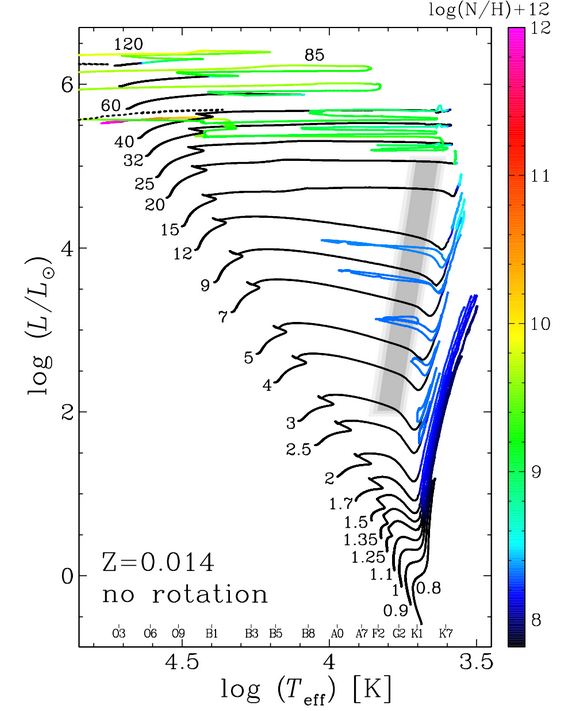
\includegraphics[width=0.65\textwidth]{intro/HRD}
 \caption[HRD]{
H-R diagram displaying evolutionary tracks of stars in the mass range 0.8~$<$~M/M$_{\odot}$~$<$~120 taken from
\protect\citet{2012A&A...537A.146E}.
 \label{fig:HRD}}
\end{figure}


During core hydrogen-burning, stars more massive than 1.1M$_{\odot}$ fuse hydrogen to helium through the carbon$-$nitrogen$-$oxygen (CNO) cycle.
In this case, convection is induced owing to the large temperature gradient established as a result of the high temperature dependence of the rate of the CNO cycle (T$^{14}$).
As a result of convective mixing, the core can be described as homogeneous during the hydrogen-burning phase~\citep{b:KippenhahnWeigert}.
Convection is an important feature of this stage of evolution as it increases the MS lifetime by increasing the amount of material available for fusion.

Some of the main issues with the current theory of convection are characterising the size of the convective overshoot region and the effects of semi-convection on stellar evolution.
Convective overshooting acts to increase the mixing of material beyond the convective boundary, within a stable region.
As a convective cell is accelerated towards the boundary of the convective layer, its momentum carries the cell beyond this region into a region of convective stability.
This has several consequences for the evolution of the hydrogen-burning phase, which are direct results of convective overshooting increasing the amount of fuel available for consumption within the convective core.
How large an evolutionary effect convective overshooting produces is not well constrained.

Convective overshooting is characterised by the parameter $\alpha$ in units of the local pressure scale height ($H_{P}$)~\citep{b:KippenhahnWeigert}.
% What is the local pressure scale height?
Various authors have placed constraints upon $\alpha$ by using observational techniques including, for example, measuring the width of the main sequence~\citep{Schroder97,Brott11}.
These studies (along with many others) find values of $\alpha$ = 0.1$-$0.6~\citep[a recent example is][finding $\alpha = 0.335$]{Brott11}.
%[measuring the width of the MS get us constraints on alpha? Model the overshooting predicts larger radii and hence greater luminositiies. Using eclipsing binaries allows us to accurately measure the mass and radii of stars on the MS]
% What does a \alpha = 0.335 actually mean?

Semi-convection is also an issue for more massive stars.
This is because, in massive stars, opacity is dominated by electron scattering~\citep{b:Bohm-vitense92.v3}.
Semi-convection is named as such because of a discrepancy between two different criterion for convection.
This situation arises outside a fully convective zone where a chemical gradient ($\nabla _{\mu}$) is established.
Semi-convection acts to smooth out the chemical gradient outside the fully convective regions.
% [This is not a good explanation of semiconvection!]
% What implications does semi-convection have for massive stars?
% Why does semi-convection only occur in massive stars on the MS?
%% In massive stars the opacity is dominated by electron scattering
%%
%% convection occurs if the radiatve temperature gradient exceeds the adiabatic temperature gradient


As the star evolves and more hydrogen is consumed, the mass of the convective core decreases~\citep{b:KippenhahnWeigert}.
Eventually, the star consists of a pure helium core surrounded by a hydrogen-burning shell.
The maximum mass of the helium core, with respect to the total stellar mass is determined by the Sch\"onberg$-$Chandrasekhar limit (q$_{SC}$ $\geq$ $\frac{M_{c}}{M_{tot}}$; usually derived as q$_{SC}$ $\sim$ 0.1), above which an inert helium core is unstable to gravitational collapse.
In stars in the mass range 3 $<$M/M$_{\odot}$ $<$ 12, the Sch\"onberg$-$Chandrasekhar limit is usually reached at the end of the hydrogen-burning phase~\citep{b:SalarisCassisi05}.
At this point, the helium core collapses, increasing the core temperature and density sufficiently that core helium-burning can occur, halting the collapse in the process.
In more massive stars ($>$ 12$M_{\odot}$), core helium-burning can smoothly proceed without the need for core collapse, as the central temperature in these stars is sufficiently high (10$^{8}$K).

During this phase of evolution hydrogen-burning proceeds within a shell outside the core.
For stars which exceed the Sch\"onberg$-$Chandrasekhar limit, during core contraction the outer hydrogen envelope will expand owing to the \textquoteleft mirror principle\textquoteright ~of shell fusion.\footnotemark
\footnotetext{This principle is not well understood, but its effects appear to be a universal feature of shell fusion.}
As the outer envelope expands, the effective temperature decreases.
In Figure~\ref{fig:HRD}, the star moves to the right (towards redder colours) where massive stars evolve into the RSG phase and lower mass stars become red giant branch stars.
This phase of evolution proceeds on a Kelvin$-$Helmholtz timescale, which for a 7M$_{\odot}$ star is around 5$\times$ 10$^{5}$years~\citep{b:KippenhahnWeigert}, i.e. incredibly short on an evolutionary timescale.
The short timescale on which this evolutionary phase proceeds accounts for the observed Hertzsprung gap.
The evolution towards the red is halted as core helium-burning switches on.

In massive stars above 12M$_{\odot}$, core helium-burning is thought to ignite when the star appears as a blue supergiant (BSG)~\citep{Meynet11,2012A&A...537A.146E,Langer12,Saio13}.
The redward migration of BSG stars is dictated by an intermediate convective zone~\citep{Meynet11} present in the atmosphere of the star, and is more gradual than the redward evolution of less massive stars.
Stars more massive than around 40$M_{\odot}$ never become RSGs~\citep{Massey03,Meynet11,2012A&A...537A.146E} and hence, there is a peak luminosity of RSGs in any given population.
As these massive stars evolve towards the red edge of the Hertzsprung$-$Russell (HR) diagram, their luminosities approach that of their Eddington luminosities; this induces large mass loss episodes.
As a result, these stars halt their evolution towards the RSG phase and evolve towards the blue and consequently into Wolf$-$Rayet (WR) stars~\citep{Crowther07, Vink09}, see 60M$_{\odot}$ track and above in Figure~\ref{fig:HRD}.

For a 10M$_{\odot}$ star, core helium-burning proceeds for around 4Myrs~\citep{b:SalarisCassisi05}.
As suggested above, in specific cases, not all of the helium-burning phase is spent as a RSG.
The length of time spent during the RSG phase depends upon how core helium-burning ignites.
If a star begins its helium-burning lifetime as a BSG and subsequently evolves into the RSG phase, naturally, the length of time spent as a RSG will be shorter.
In addition to this, stars with masses in the range of 25$<$M/M$_{\odot}$ $<$40 are thought to evolve back from the RSG phase to the BSG phase while still burning helium in their cores~\citep{2012A&A...537A.146E}.

This evolution of massive stars between the BSG and RSG phase seeds the idea that stars in these stages of evolution will fall into two categories:
(i) stars which begin helium-burning in the RSG or BSG phase, or (ii) stars which began helium-burning in a different evolutionary state and have since evolved into either the RSG or BSG regime.
Distinguishing these objects observationally is challenging.
\cite{Saio13} use radial pulsations to distinguish between models of BSGs, which \textquoteleft roughly agree\textquoteright ~with observations of NGC 300 and in the Galaxy.
However, an analogue to this has not been identified in RSGs.

% Convection has a big role to play here.
%% Stellar models based on the Schwartzchild criteria for convection spend more time in the blue compared to models based on the Ladaux certeria~\citep{SalarisCassisi05}
% More about mass loss from BSGs

Regardless of how extended the external envelopes in these stars are, core helium-burning proceeds in an identical manner.
Helium burning in general proceeds through the triple alpha process, via the reaction, 3$\alpha$ $\rightarrow$ $^{12}$C+$\gamma$.
However, as the number density of $^{12}C$ increases, the reaction $^{12}$C($\alpha$+$\gamma$)$^{16}O$ is of increasing importance, although the exact rates at which these reactions proceed is not well constrained.
This process of nuclear burning is highly temperature sensitive (even more so than the CNO cycle); therefore, a convective core is once again induced.
In addition to this, massive red helium-burning stars also have large outer convective envelopes~\citep{b:KippenhahnWeigert}, which means the star appears near the Hayashi limit for a fully convective star in the HR diagram.
The convective envelope dominates the evolution of all but the most massive RSGs (30$<$ M/M$_{\odot}$ $<$40) which do not not appear as close to the Hayashi limit as their lower mass counterparts~\citep[see Figure 1 in][]{Saio13}.


%The size of the convective outer envelope increases with the mass of the star~\citep{b:KippenhahnWeigert}.
%The structure of a helium-burning massive star also consists of the hydrogen-burning shell at the boundary of the convective envelope and convective core.
%This hydrogen-burning shell contributes significantly to the overall energy output of the star during the helium-burning phase of evolution.
%% Hertzprung gap?
% Large mass loss rate of RSGs favour a blueward evolution~\citep{Salasnich99, Ekstrom11}


%% No observational evidence that stars directly evolve to RSG from the MS ...~\citep{Langer12}
%% El Eid 1995 \& Langer \& Maeder 1995 show that massive stars can ignite helium in BSG phase before evolving towards the RSG stage (see also Ekstrom + 2008)
%% in stellar evolution codes, depending upon choices of parameters for convection, semi-convection and overshooting, stars can begin he-fusion in the BSG phase ref's ^^^
%% BGS have  a population of Case B mass transfer stars with an under-massive helium core
%% No clear gap between BSGs and MS stars~\citep{Hunter08, Langer12}
%% Low rotational velocity of BSGs~\citep{Vink+10}
%% Humphreys \& Davidson 1979, 1994 upper limit on Galactic RSG luminosity logL/L$_{\odot}$ = 5.8
%% More luminous stars reach Eddington luminosity before reaching the RSG stage due to an increased opacity of the outer layers of the star~\citep{Langer12}


At the end of the core helium-burning phase, a massive star contains a carbon/oxygen core surrounded by a helium-burning shell, which is in turn surrounded by a hydrogen-burning shell.
At this point, the situation in the core now resembles that of the stage before core helium-burning.
An inert carbon/oxygen core contracts and heats up which ignites the core fuel.
Stars with initial masses greater than around 8M$_{\odot}$ are able to fuse carbon in their cores in a stable fashion.
In order for lower mass stars to do so, a degenerate carbon core is required.
Whether or not stars are able to begin core carbon-burning in a stable manner is usually the physical basis for distinguishing between \textquoteleft  intermediate\textquoteright ~and \textquoteleft high\textquoteright ~mass stars.
During this process, carbon fuses to form an unstable form of $^{24}$Mg which then decays through three channels: (i) $^{24}$Mg$^{*}$$\rightarrow ^{23}$Mg$ + n + \gamma$, (ii) $^{24}$Mg$^{*}$$\rightarrow$$^{20}$Ne+$\alpha$+$\gamma$, (iii) $^{24}$Mg$^{*}$$\rightarrow$$^{23}$Na+p+$\gamma$.
Oxygen does not fuse at this stage of the evolution of the star and therefore the length of time a star spends fusing carbon depends strongly on the amount of carbon processing present in the helium-burning phase (namely, the reaction $^{12}C(\alpha+\gamma)~^{16}O$).

Once the carbon fuel has been exhausted in the core, shell carbon-burning proceeds.
The cycle of core contraction with new core reactants begins and subsequent neon-, oxygen- and silicon-burning in the core follow~\citep{Woosley02}.
As each new fuel in the core is exhausted, subsequent shell burning follows.
Fusion reactions cease with $^{56}$Fe as fusion reactions beyond this point are no longer energetically favourable.

Eventually, this leads to an \textquoteleft onion structure\textquoteright
~star, with an inert iron core surrounded by layers of lighter elements fusing in shells.
These fusion reactions proceed on such a short timescale that the outer envelope does not have the time to react to the changing conditions in the core.
This effectively \textquoteleft freezes out\textquoteright ~the outer envelope and the spectral type of the star does not change significantly during this period~\citep{Meynet11}.

% Factors affecting this evolution:
%% MASS LOSS!!!
%% Binarity

%% Various notes on this section
% STars can migrate back towards the blue if the mass of the He core reaches around 60-70% of the total mass~\citep{Meynet11, Giannone67?}
% Evolving blueward depends upon the mass loss and mixing~\citep{Meynet11}
% Strong mass loss favours blueward evolution (Yoon & Cantiello 2010, Vanbeveren, Van Bever & belkus 2007, Salasnich + 1999)
% Strong mixing also increases the mass of the He core (Hirschi+2004)

% In general more massive stars spend less time on the MS t=E/L assume same fraction of the total mass is consumed in all stars, therefore E proportional M,  t~M/L tpyically L~M^3.5, t~M^-2.5
% From models of stellar evolution of stars greater than 10 solar masses have a lifetime of around $<30$Myrs~\citep{Crowther12}, which means in relative terms, they are very young objects.

% Consequences of overshooting: longer MS lifetime as more material can be used, larger increase in Luminosity on the MS, Larger helium core at the end of core hydrogen fusion
%% Convective cells are accelerated towards the boundary until they reach this boundary and the acceleration is switched off

% semiconvection affects the region external to the convective zone and can act to increase mixing in this zone.
% Hydrogen shell burning usually occurs through the CNO cycle~\citep{b:SalarisCassisi05}

%Measurements of Galactic RSGs have yielded radii of up to $1500M_{\odot}$~\citep{something about beteguese or that other one ... VY CMa?}


%% Distinction between low mass, intermediate mass and high mass stars

% Low mass 0.8 < M < 2 M_{\odot}: Fuse helium in a degenerate core, go through a helium flash

% Intermediate mass 2 < M < 8: Fuse helium in a stable manner. No helium flash. Fuse Carbon via a degenerate core

% Massive stars 8+ Fuse Carbon in a stable manner

% subsection life_cycle (end)

\subsection{Death} % (fold)
\label{sub:death}

Massive stars ($>$8M$_{\odot}$) end their lives as core-collapse supernovae (CCSN).
These violent explosions are responsible for distributing elements synthesised within massive stars during their nuclear-burning lifetime, as well as during the explosion event.
Observationally, CCSN are classed as type II, type Ib and type Ic.\footnotemark
\footnotetext{Type Ib and type Ic are often grouped as type Ibc, as the differences between these two types are difficult to distinguish~\citep[for example see][]{Eldridge13}.}
The classification of supernovae (SNe) is based on their optical spectra, specifically on the appearance of spectral features such as hydrogen and helium.

There are several different types of CCSN which occur as a result of the different conditions present in the cores of massive stars.
For an in depth review see~\cite{Janka12}.
For the purpose of this literature review, it will suffice to mention the four main CCSN channels: electron-capture SNe, iron-core SNe, gamma-ray burst SNe and pair-instability SNe.
This review will focus on iron-core SNe in particular.

Iron-core SNe account for the majority of observed CCSN~\citep{Smartt09,Janka12,Eldridge13}.
This type of SNe are produced by massive stars which have initial masses above $\sim$9M$_{\odot}$~\citep{Poelarends08}.
As mentioned in the previous section, massive stars conclude their nuclear-burning lifetimes with inert iron cores.
Owing to a lack of energy generation, the core contracts and heats up.
As the temperature reaches 10$^{10}$K, photons in the core of the star now have enough energy to photo-dissociate iron-group elements into $\alpha$ particles.
The increasing density forces electrons into nuclei and free protons, creating a neutron rich environment.
As densities approach nuclear density, core contraction halts as a result of the repulsive force of the strong interaction~\citep{Janka12}.
The in-falling outer layers crash into the core and the resulting shock-wave disrupts the entire star and produces the SN.

The exact mechanism which produces the SN explosion is subject to intense research, the subtleties of which will not be covered in this literature review.
Recently, two extensive review articles~\citep{Janka12, Burrows13} have been published on the subject giving a more in depth and complete overview of the subject.

In recent years, many SN progenitors have been discovered by reviewing extensive archival data available in the Local Group as well as through extensive dedicated SN surveys.
These studies (or a quick review of the Central Bureau for Astronomical Telegrams (CBAT) list of SNe\footnotemark) reveal that type II-P SNe are by far the most numerous type of CCSNe ($\sim$ 60\%) and RSG stars are firmly established as their progenitors~\citep[][and references therein]{Smartt09}.
\footnotetext{http://www.cbat.eps.harvard.edu/iau/cbat.html}
However, CCSN are observed in a variety of different types and hence, RSG stars are not the only type of massive star which can end their lives as SNe.
Figure~\ref{fig:SNe-Smartt} illustrates the many possible channels towards SNe; this includes RSGs, BSGs, WRs and recently luminous blue variable (LBV) stars are being established as a part of this list~\citep[e.g.][]{Smartt09, Groh13}.

% \begin{figure}
  % \begin{center}
 %  \epsfxsize=150mm         % Horizontal size YOU want
 %  \epsffile{Smartt09fig12.eps}
 %  \caption{The evolutionary diversity of the end points of massive stars and their associated observed SN classification. Figure reproduced from~\cite{Smartt09}. Acronym definitions: RSG, red supergiant; BSG, blue supergiant; LBV, luminous blue variable; WR, Wolf$-$Rayet; NS, neutron star; BH, black hole; GRB, gamma-ray burst; PISN, pair-instability supernova.}
 %    \label{SNe-Smartt}
 %    \end{center}
 % \end{figure}

 \begin{figure}
 \centering
 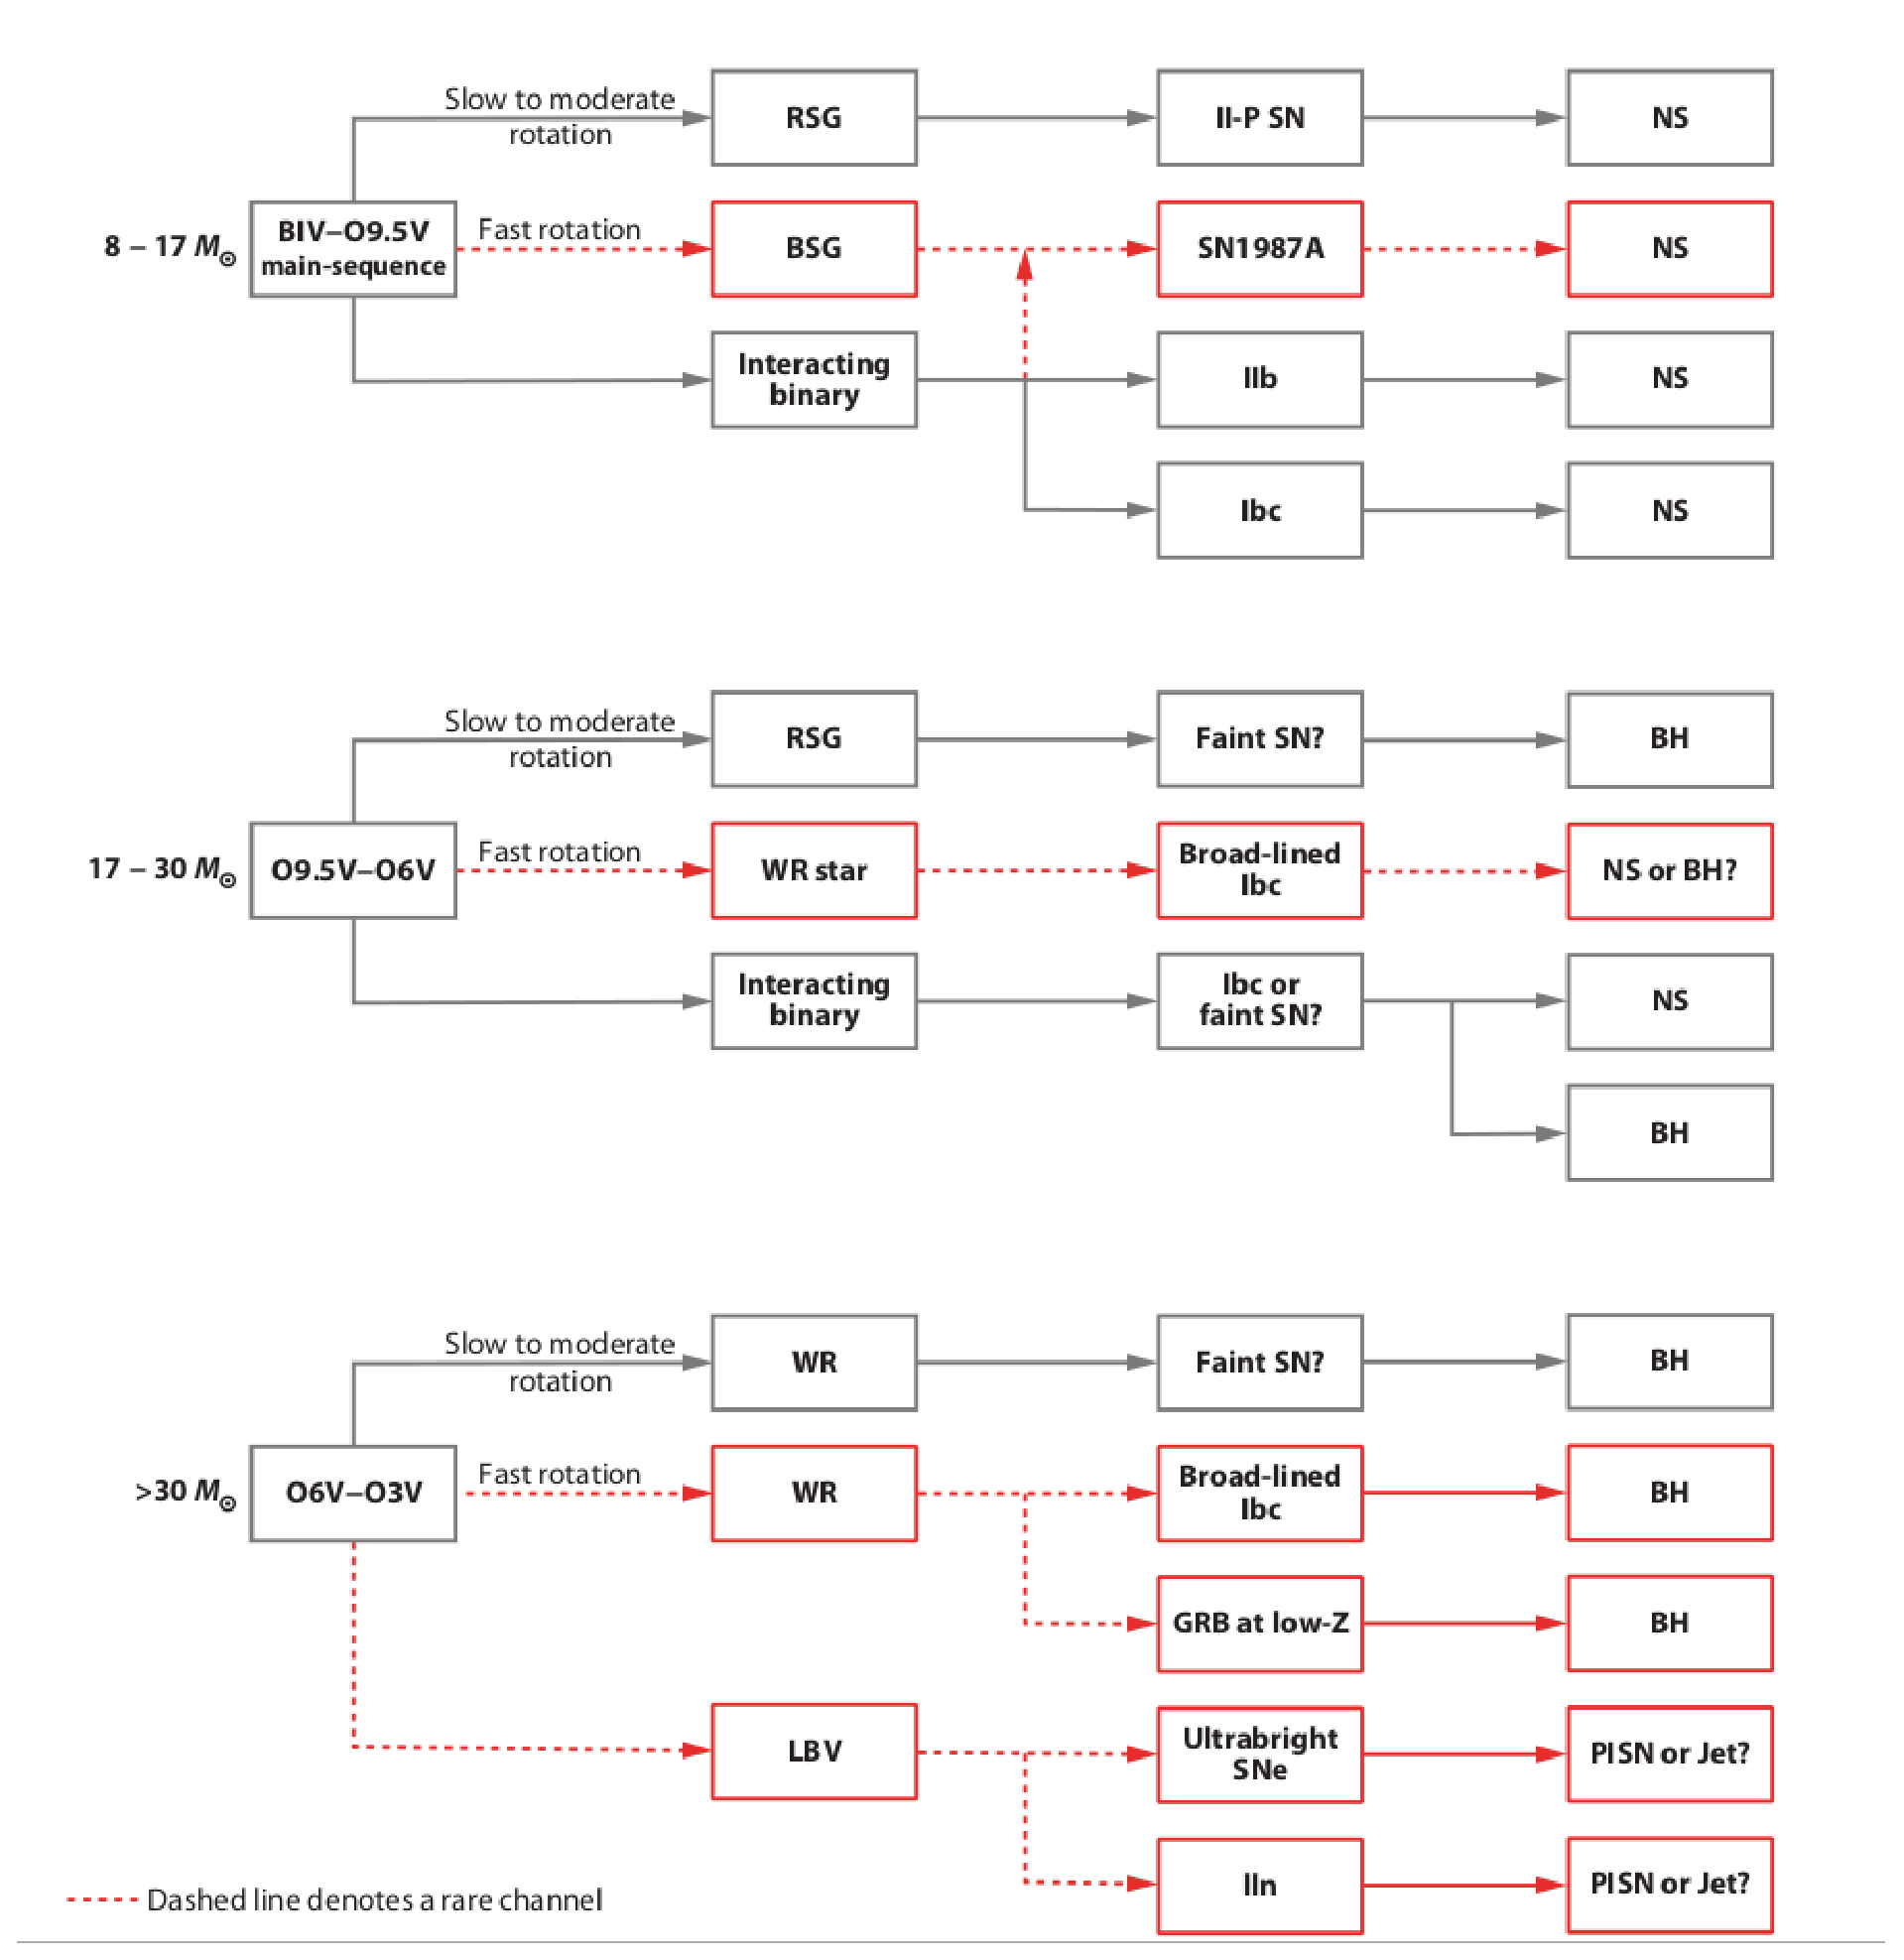
\includegraphics[width=0.65\textwidth]{intro/Smartt09fig12}
 \caption[HRD]{The evolutionary diversity of the end points of massive stars and their associated observed SN classification. Figure reproduced from~\cite{Smartt09}. Acronym definitions: RSG, red supergiant; BSG, blue supergiant; LBV, luminous blue variable; WR, Wolf$-$Rayet; NS, neutron star; BH, black hole; GRB, gamma-ray burst; PISN, pair-instability supernova.
 \label{fig:SNe-Smartt}}
\end{figure}

% subsection death (end)
% section the_life_of_a_red_supergiant (end)

\section{Chemical Properties of Red Supergiants} % (fold)
\label{sec:chemical_properties_of_red_supergiants}

\subsection{{\it J}-band Analysis Technique} % (fold)
\label{sub:subsection_name}

% subsection subsection_name (end)
\subsection{Galactic and Extragalactic RSGs} % (fold)
\label{sub:galactic_and_extragalactic_rsgs}

The intrinsic brightness of RSGs, particularly in the NIR, makes these stars popular candidates for observations within and beyond the Galaxy.
Studies of Galactic RSGs are used to derive fundamental stellar parameters such as radii, masses and distances.
Galactic RSGs are also a natural starting point for extragalactic studies of larger populations of RSGs.
Extragalactic observations have identified populations of RSG stars in a large range of galaxies within the Local Group and (in rarer cases) out to larger distances~\citep[e.g.][]{Elias85,Humphreys86, Massey06, 2007AJ....134.2474M, Groenewegen09,Massey13}. % how do I put "table 1 in massey"?
These studies provide important results on RSGs in different environments.
To illustrate this, this section first comments on some of the fundamental parameters derived using Galactic RSGs in Section~\ref{Galactic RSGs} and summarises some of the important observational results regarding extragalactic RSGs in Section~\ref{extragalactic RSGs}.
In Sections
\ref{selection} and
\ref{Galactic RSGs}, I focus on some of the aspects of extragalactic RSGs which will be applicable in later stages of this document.

\subsubsection{Fundamental Parameters in Galactic RSGs}\label{Galactic RSGs}

Research into Galactic RSGs is typically divided into two categories: studies of individual nearby stars such as Betelgeuse~\citep[$197\pm 45$pc;][]{Harper08} and VY CMa~\citep[$1420\pm$ 120pc;][]{Wittowski12} and studies of populations of RSGs within open clusters and associations~\citep[e.g.][]{Levesque05,Negueruela13}.
Studies of individual Galactic RSGs concentrate on the fundamental parameters of these stars such as their distances, mass-loss rates and circumstellar envelopes.
Additionally, nearby Galactic RSGs are tests for detailed stellar atmosphere and evolutionary models.

Observations of Galactic RSGs reveal that they have large mass-loss rates~\citep[10$^{-(6\pm 1)}$M$_{\odot}$yr$^{-1}$;][]{Danchi94, Richards13} and extended circumstellar environments~\citep{Smith01} which may containing masers~\citep{Schuster06}.
Mass loss during this phase of evolution is critical for the understanding of subsequent evolutionary stages as well as understanding SN progenitors.
%The remnant of SN 1987A displays loops which are thought to have origionated in mass loss events during the RSG phase of evolution of its progenitor star~\citep[][and references therein]{Humphreys13}.
Galactic RSGs act as an important sample to study and understand the mechanisms of mass loss, as extragalactic observations are unable to resolve the structure which can be seen in nearby Galactic stars.

One of the main uncertainties with studies of these nearby stars are the relatively poorly constrained distances (e.g., Betelgeuse with a distance uncertainty of nearly 25\%).
In order to (partially) remove the distance uncertainty problem, RSGs can be observed in Galactic clusters of known distances~\citep[e.g.][]{Humphreys78, Mel'Nik95}.
%% MS fitting, observe spectral type and fit cluster onto a HR diagram to estimate the absolute magnitude, distance modulus
This technique is useful to study large populations of RSGs which can be used to test theories of star formation and models of RSGs and their atmospheres.
Studies of RSGs in Galactic clusters are often used as a first test for studies which plan to include observations at larger distances~\citep[e.g.][]{Levesque05,Levesque06, 2010MNRAS.407.1203D,2013ApJ...767....3D}.

\subsubsection{Extragalactic Studies and Results}\label{extragalactic RSGs}

Extragalactic studies of RSGs are advantaged in that it is possible to accumulate large samples of RSGs with which to test stellar evolution theories and derive stellar parameters.
By using the different environments available in the Local Group, studies of extragalactic RSGs can probe a wide range of host galaxy parameter space.
For example, M31 (Z$>$1.0Z$_{\odot}$ in the central regions), a massive, metal-rich spiral galaxy and the Wolf$-$Lundmark$-$Melotte (WLM; Z=0.1Z$_{\odot}$), a dwarf irregular, metal-poor galaxy, both contain a significant population of RSGs.

Through an analysis of RSGs in different metallicity environments, various authors report that the average spectral type of a RSG population is dependent upon metallicity~\citep{Elias85, MasseyOlsen03, 2012AJ....144....2L}, where lower metal abundances give rise to earlier average spectral types.
%% Chris' comment:
%not necessarily - the way I always thought about this was that, e.g., in the SMC, the TiO bands are weaker, so for a given spectral type, the star needs to be cooler to reproduce the TiO strengths for, e.g. M3 or M4 types.  Thus, the coolest star could have the same Teff, but its spectral type will appear earlier.
In addition to this, RSGs can be used to measure abundances in Local Group galaxies, which yield important results by mapping metallicity gradients.
This work has typically been done using high-resolution spectra at NIR wavelengths~\citep{Cunha07, Davies09a,Davies09b}.
However, in order to optimise these studies,~\cite{2010MNRAS.407.1203D} adapted a method for determining the chemical properties of BSG stars in the optical~\citep{Kudritzki08,Kudritzki10}, to RSGs in the NIR.

Measurements of the temperatures of RSGs have also provided insight through using observations of extragalactic RSGs in the NIR.
The temperatures of RSG stars have been subject to debate for many years.
There are many methods by which to estimate the effective temperature of a RSG star.
The most popular of which is to fit the spectral energy distribution (SED) of the star with 1D model atmospheres~\citep{2008A&A...486..951G}.
However,~\cite{2013ApJ...767....3D} show that observations fitting models around the BVRI region, where molecular TiO lines dominate the absorption, result in a systematically lower temperature compared with fitting the line-free continuum regions of the SED.
This is due to the fact that the TiO molecular line forms higher in the atmosphere of the star than the continuum.
This means that fitting the TiO region and assuming that the best fitting effective temperature is representative of the entire SED is not a good assumption.
\cite{2013ApJ...767....3D} advocate using the entire SED \textit{except} those regions dominated by the TiO absorption features.
Deriving temperatures of extragalactic RSGs will be an important test for stellar evolution models and an excellent way in which to test models at different metallicities and in different environments.

In order to test models of stellar evolution against observations of extragalactic RSGs, a complete sample of RSG stars is clearly beneficial in order to draw conclusions on how the population behaves and evolves as a whole.
In order to do this, generally, stars must be selected for spectroscopic follow-up observations based on their photometric properties.
%Obviously, if an extensive stellar spectroscopic survey is available, this problem quickly disintegrates.
%However, in all other cases, photometric selection is an important factor in the study of extragalactic RSG stars.

%RSG have luminosities which can rival entire populations of stars ($> 10^{4.5-5.8}$L$_{\odot}$).
%But, unlike their hot progenitors, the peak wavelength of a RSG star is around 1$\mu$m, therefore, at NIR wavelengths, these stars dominate the light output from their host galaxies.

  % Radii, absolute magnitude ... useful?
  % Surface gravities?

  % Figure 8 from Massey 2003 and references therein
  % Figure 3 Levesque et al 2005
%% Levesque et al 2005 define a new temperature scale which brings the temperatues up
% Luminosities
% optical spectroscopy Massey, levesque, Drout etc
  % Winds/Mass loss rates
  %% Driven by radiation pressure~\citep{Langer12}
  % Rotation
%% Betelgeuse v=15kms^{-1} <-- is this a large rotation or not ... sun = 2kms^{-1}

  % Binary fraction
%% Sana et al 2012 \sim 70% of massive O stars are contained within binary systems Galactic
%% Sana et al 2013 \sim 50% of massive O stars are contained within binary systems 30 Dor (VFTS)

%% This is not true at all! circumstelalr material is very difficult to detect in RSGs (Harper et al. 2008; Smith et al.2009)
%Another property of the spectra of RSG stars which is useful in order to distinguish these objects from their lower mass counterparts is the presence of emission lines.
%These lines arise due to the circumstelar material surrounding all RSG stars.
%This circumstellar material arises from the strong winds which are characteristic of all RSGs and will be discussed further in Section~\ref{properties}.

\subsubsection{Photometric Selection of RSGs}\label{selection}

In the absence of spectroscopic observations, the selection of objects with respect to follow-up observations is often done using broad band photometry.
%Broad band observations typically use the standard Johnson-Cousins filters, UBVRIJHK(K$_{s}$).
This section will describe some of the various methods used to isolate a population of stars using magnitudes derived from broad band filters.
This is important as good photometric selection of targets can optimise observing strategies and should be able to provide a complete sample of the population of stars.

Colour$-$magnitude diagrams (CMDs) are often used to isolate a particular type of star.
A colour is defined as the difference between two magnitudes, derived from  two different filters, and colours trace the temperature of a star (and hence their spectral type), whereas magnitude can be used to approximate luminosity.
Therefore, using CMDs should allow the separation of a population of red, luminosity class I (supergiant), stars.
However, using this method assumes that the sample consists purely of one population of stars at a given distance; if this assumption is not true, apparent magnitude is no longer sensitive to luminosity.
For example, a nearby population of faint stars with similar spectral types (colours) could pose as a bright population of more distant objects.
This becomes important when viewing an extended extragalactic object, such as a stellar cluster or external galaxy, at low Galactic latitude where the Galactic stellar density is highest.
An example of a typical CMD is given in Figure~\ref{fig:CMD}.

 \begin{figure}
 \centering
 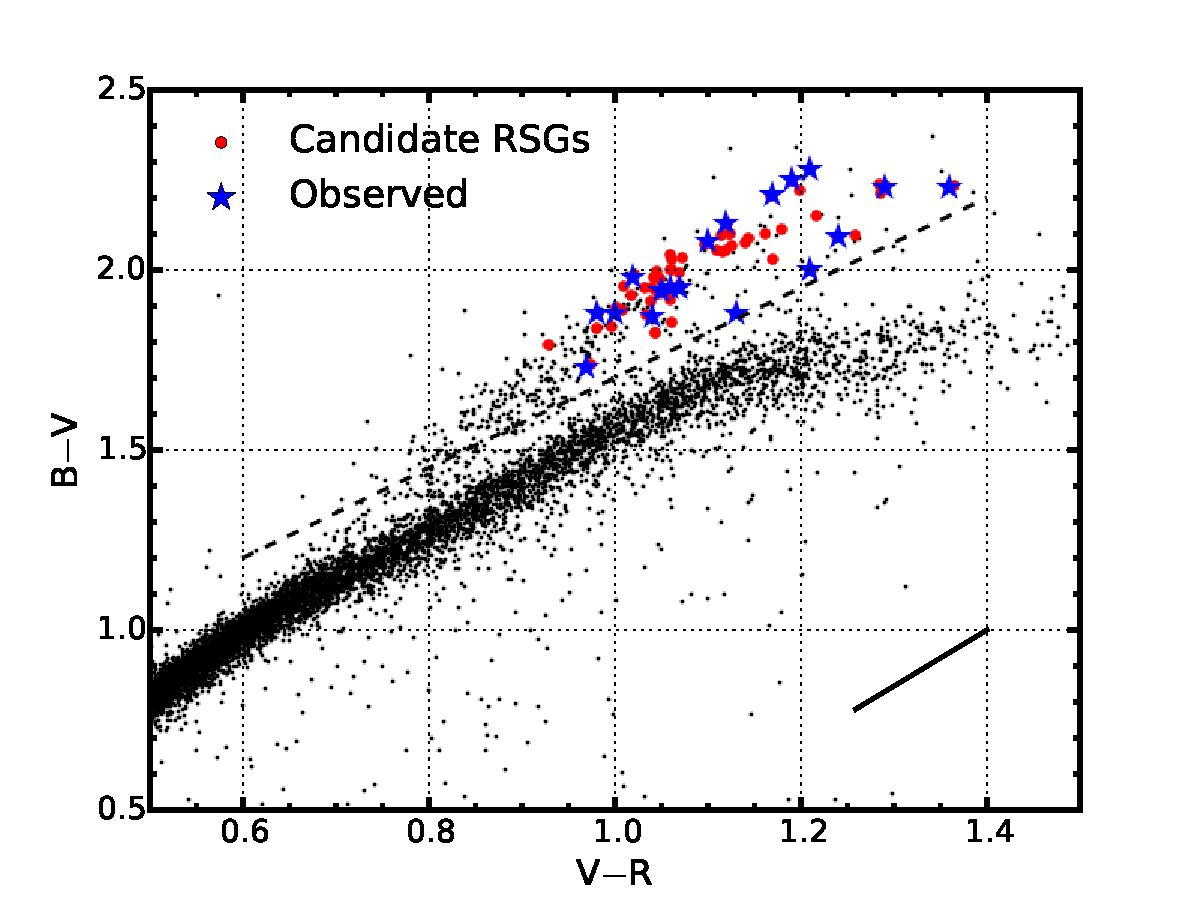
\includegraphics[width=0.65\textwidth]{intro/N6822_bvr}
 \caption[B$-$V, V]{Optical colour-magnitude diagram (CMD) of NGC 6822, in which the absolute V-band magnitude M$_{V}$, (corrected to the distance of NGC 6822) is plotted against B$-$V colour.
This figure illustrates how CMDs can be used to separate stars based on spectral type. Redder colours indicate later spectral types.
This figure also demonstrates that CMDs have inherent degeneracies  between different populations of stars: the central dense feature at B$-$V $\sim$ 1.0 is attributed to foreground contaminants
 \label{fig:CMD}}
\end{figure}

% \begin{figure}[t]
%   \begin{center}
%   \epsfxsize=150mm         % Horizontal size YOU want
%   \epsffile{bvcmd_all_example.eps}
%   \caption{Optical colour-magnitude diagram (CMD) of NGC 6822, in which the absolute V-band magnitude M$_{V}$, (corrected to the distance of NGC 6822) is plotted against B$-$V colour.
% This figure illustrates how CMDs can be used to separate stars based on spectral type. Redder colours indicate later spectral types.
% This figure also demonstrates that CMDs have inherent degeneracies  between different populations of stars: the central dense feature at B$-$V $\sim$ 1.0 is attributed to foreground contaminants.}
%     \label{CMD}
%     \end{center}
%  \end{figure}
 \begin{figure}
 \centering
 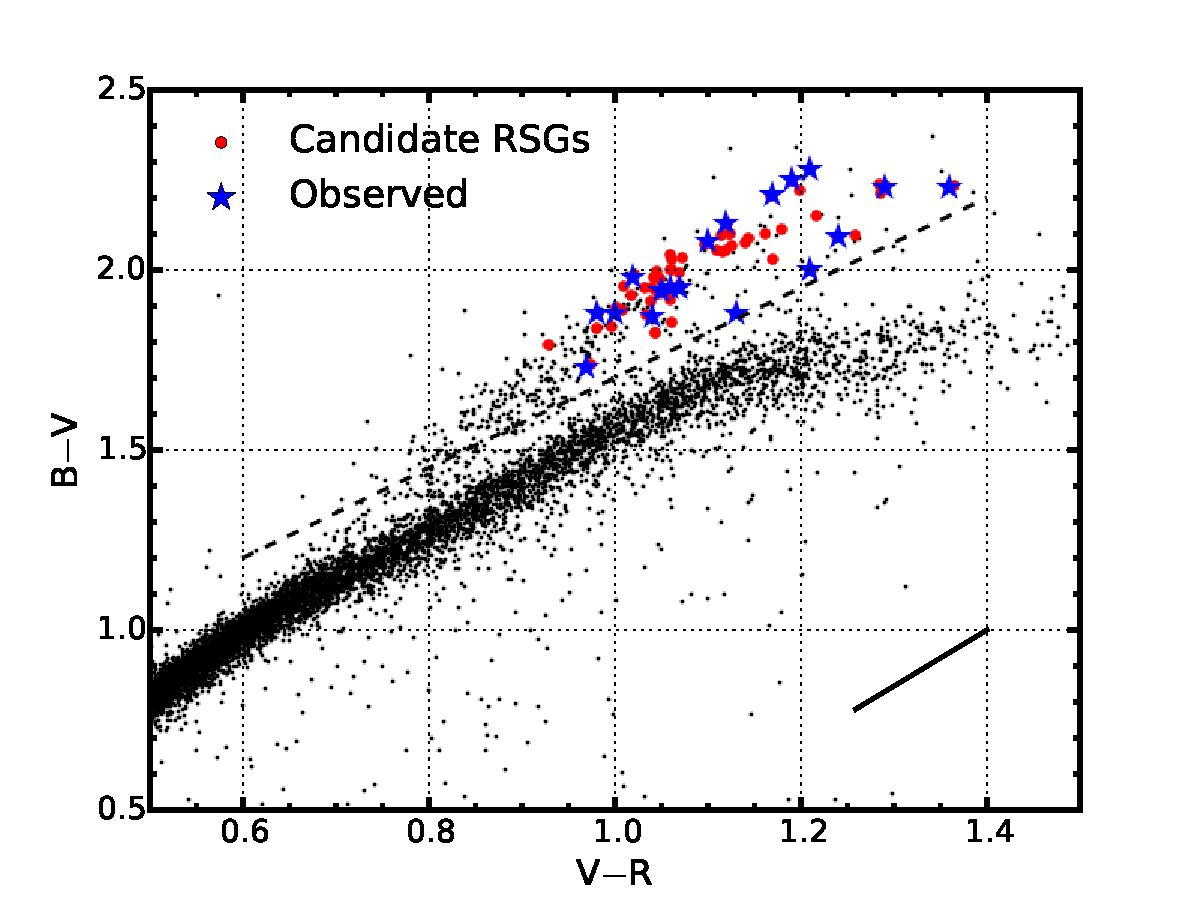
\includegraphics[width=0.65\textwidth]{intro/N6822_bvr}
 \caption[B$-$V, V$-$R]{Optical colour$-$colour diagram of NGC 6822. This figure illustrates the surface gravity dependence of the B$-$V colour at a given V$-$R colour. The population with the redder B$-$V colours contain the RSG objects.
 \label{fig:CCD}}
\end{figure}

% \begin{figure}[t]
%   \begin{center}
%   \epsfxsize=150mm         % Horizontal size YOU want
%   \epsffile{bvrccd_example.eps}
%   \caption{Optical colour$-$colour diagram of NGC 6822. This figure illustrates the surface gravity dependence of the B$-$V colour at a given V$-$R colour. The population with the redder B$-$V colours contain the RSG objects.}
%     \label{CCD}
%     \end{center}
%  \end{figure}

To break the degeneracy between luminosity and distance, one can use colour$-$colour diagrams.
Using multiple colour diagnostics can isolate stars based on more than just spectral type and absolute magnitude.
\cite{1998ApJ...501..153M} show that at a given V$-$R colour, the B$-$V colour is sensitive to the surface gravity of a star.
Therefore, given a V$-$R colour, RSGs can be isolated owing to their low surface gravity.
An example of such a colour$-$colour diagram is shown in Figure~\ref{fig:CCD} where one can clearly see the distinction between low surface gravity RSG stars (with slightly redder B$-$V colours) and the dwarf high surface gravity stars.

The selection of RSGs is typically done using a B$-$V, V$-$R colour$-$colour diagram as this diagram has had much success in selecting RSGs and is known to contain a small number of contaminants.
However, a potential issue with these diagrams as we move to extragalactic systems, which at the time of writing has not been quantified, is that RSGs are known to reside in dense regions and/or clusters with many bluer, younger stars.
When viewing these stars in the optical, the colours from RSGs could potentially be contaminated to bluer colours by the blue stars which also reside nearby.
In a B$-$V, V$-$R diagram, this contamination would affect the completeness of the population of RSGs selected.
As stated, this is not quantified and would require a comparison between the B$-$V, V$-$R selection method with another known selection method and an analysis of the locations of the potentially contaminated RSG stars.
A potential solution to this problem would be to select RSGs based on their NIR colours, which is where these stars are brightest and hence would be less subject to contamination to nearby blue objects.
% This argument could be reversed and in the NIR we could push blue stars towards our RSG targets. Would this be a problem?

Working in the NIR, authors have used the J, J$-$K CMD~\citep{2000ApJ...542..804N,2006A&A...452..195C,Neugent12} to select red stars (RSGs and asymptotic giant branch (AGB) stars) and much work has been done in identifying contaminants and the parameter space where individual populations reside in~\citep{2006A&A...452..195C}.
As mentioned above, the main contaminants with this selection method are foreground dwarfs.


% subsection galactic_and_extragalactic_rsgs (end)
% section chemical_properties_of_red_supergiants (end)

\section{Chemical Evolution of Galaxies} % (fold)
\label{sec:chemical_evolution_of_galaxies}

The evolution of galaxies is a vast field and can be broadly split up into three main fields: dynamical, thermal and chemical evolution.
%In reality these topics depend upon each other, but given certain crude approximation can to an extent be studied independently.
The chemical evolution of galaxies governs the origin and distribution of elements within the host galaxy.
This evolution principally depends upon galaxy and star formation.
The initial origin and distribution of the chemical elements depends upon the galaxy formation process.
Star formation acts to alter these quantities by creating, redistributing and removing chemical elements from the interstellar medium (ISM).

The lowest mass stars remove elements from the ISM by storing their gas and never evolving off the MS!
Stars massive enough to evolve off the MS eject some mass during an AGB phase, but subsequently end their lives by removing elements from the ISM as passively cooling white dwarf stars.
%These stars could also end up as Type Ia SNe
More massive stars undergo large amounts of mass loss during all phases of their evolution and end their lives by exploding as CCSNe, both of which act to alter the chemical composition of their surrounding gas clouds.

All three of these processes are important to take into account when studying how galaxies chemically evolve over time.
However, quantifying contributions from these quantities is an involved process, complicated by a minefield of caveats and uncertainties.

Extragalactic observations of fundamental properties of galaxies play important roles in refining theories of galaxy formation and evolution.
The mass$-$metallicity relationship~\citep[MZR;][]{Lequeux79} of galaxies combines two fundamental parameters of galaxies.
The stellar mass represents the amount of gas which star formation has removed from the ISM, whereas the present day galaxy metallicity represents how star formation has altered the initial ISM.
Various authors have shown that galaxy mass is proportional to metallicity~\citep{Tremonti04, Maiolino08,Kewley08}.
This relationship can be interpreted by considering multiple factors.
In low-mass galaxies, outflows and SNe have a greater affect on the amount of material ejected from the host galaxy into the intracluster medium, owing to their shallower potential wells~\citep[e.g.][]{Tremonti04}.
Additionally, low-mass galaxies represent an early stage in Galactic evolution and hence, these galaxies have not had time to process their gas into stars.
As the host galaxy evolves, subsequent episodes of star formation increase the metal content of the galaxy~\citep[e.g.][and references therein]{Maiolino08}.

MZR observations have typically relied upon ratios of strong oxygen emission lines (usually [OII], [OIII] relative to H$\beta$) from HII regions to derive metallicities of individual galaxies.
This technique is used due to its applicability over a large distance range:
\cite{2001MNRAS.323..887C} use this technique in nearby galaxies whereas \cite{Maiolino08} derive metallicity using this method in galaxies at z$>$3.
However, these measurements are known to be highly dependent upon the calibration method used~\citep{Kewley08, Kudritzki08,Bresolin09}.
In order to provide an independent calibration of this method, BSG stars have been used to determine metallicity and abundance gradients in external galaxies~\citep{Kudritzki12}.
In addition to this,~\cite{Davies13b} outline a method using RSGs as abundance probes with which to calibrate the MZR.
These authors show that using a NIR window around 1.2$\mu$m (J-band) the dominant spectral features are that of strong metallic lines of iron and alpha elements (Ti, Mg, Si).
These strong metallic lines allow abundance measurements from relatively low resolution spectra meaning that this technique can be used at distances of 3-4Mpc with an 8-10m class telescope (significantly, outside the Local Group).


Another advantage of using relatively low resolution spectra are that multi-object spectrographs can be used to observe extragalactic systems.
This provides not only reliable abundances in nearby galaxies but also spatial information about abundances in these galaxies which allows the determination of metallicity gradients.

Therefore, extragalactic observations of RSG stars are important in order to provide independent constraints on some of the fundamental properties of Galactic formation and evolution.
These studies have enormous potential in the era of extremely large telescope era which will be optimised for NIR observations.
% section chemical_evolution_of_galaxies (end)
